\chapter{Implementazione}
L'obiettivo di questo capitolo è quello di sviluppare un'implementazione in linguaggio C per l'algoritmo basato sul
metodo di Frank-Wolfe che risolve il rilassamento lineare del set-covering. Inoltre, presenteremo anche il codice
necessario a risolvere le istanze del problema con l'algoritmo del simplesso, che verrà usato per operare un confronto
nel prossimo capitolo.

\section{Generazione delle istanze}
Come anticipato in \ref{sec:refmat}, la formulazione \eqref{eq:scplr} ci permette di identificare un'istanza per il
rilassamento lineare del set-covering semplicemente utilizzando una matrice binaria di riferimento. Di
conseguenza, per creare le istanze da utilizzare con l'algoritmo risolutivo è sufficiente creare matrici binarie.

\begin{code}{adjusted title = {\pyicon\ datagen.py}}
\begin{lstlisting}[language=python, style = style, caption={Generazione delle matrici binarie di riferimento.}, label =
{lst:genmat}]
import numpy as np

def generate_matrix(m: int, n: int, p: float) -> np.ndarray:
    mat = np.random.choice([0, 1], (m, n), p=[1 - p, p])

    while True:
        nr = np.where(mat.sum(axis=1) == 0)[0]  # null rows indices
        nc = np.where(mat.sum(axis=0) == 0)[0]  # null cols indices

        if nc.size == 0 and nr.size == 0:
            break

        if nr.size > 0:
            mat[nr, :] = np.random.choice([0, 1], (nr.size, n), p=[1 - p, p])
        if nc.size > 0:
            mat[:, nc] = np.random.choice([0, 1], (m, nc.size), p=[1 - p, p])

    return mat
\end{lstlisting}
\end{code}
\noindent
La funzione appena presentata sfrutta gli strumenti della libreria numpy per generare una matrice binaria con un numero
di righe e di colonne che è specificato dai parametri {\jbm m} e {\jbm n}, rispettivamente, in cui la probabilità
di generare valori non nulli è determinata dal parametro {\jbm p}.

Dopo che la matrice è stata generata, vengono
eseguite delle operazioni per garantire che non ci siano righe o colonne interamente popolate da valori nulli. Non
vogliamo che ci siano righe nulle, poiché significherebbe avere elementi in
\(
    \mathcal{I}
\)
che non sono coperti da nessuno dei sottoinsiemi in \( \mathcal{F} \). Non vogliamo nemmeno che ci siano colonne nulle,
poichè significherebbe avere sottoinsiemi in \( \mathcal{F} \) che non contengono nessun elemento di \( \mathcal{I} \).

\subsection{Gestione dataset}
Adesso che abbiamo un modo di generare le istanze del problema, possiamo usarlo per creare dei dataset. L'idea è quella
di creare molteplici istanze dello stesso tipo, relativamente a dimensione e sparsità della matrice di riferimento, per
ottenere dei risultati più accurati.

Per ciascuna istanza di un dataset verranno memorizzati due file:
il file {\jbm mat.dat}, che memorizza la
rappresentazione dell'intera matrice di riferimento di un'istanza, e il file {\jbm csr.dat} che memorizza la
rappresentazione CSR della matrice di riferimento e della sua trasposta, insieme alle informazioni relative al numero di
righe, al numero delle colonne e al numero degli elementi non nulli. Il file {\jbm mat.dat} verrà utilizzato come
parametro di input per l'algoritmo del simplesso, mentre il file {\jbm csr.dat} verrà utilizzato come parametro di input
per l'algoritmo risolutivo basato su Frank-Wolfe. Per ottenere la rappresentazione CSR di una matrice abbiamo utilizzato
il modulo sparse della libreria scipy.

\section{Algoritmo del simplesso}
Iniziamo a presentare il codice necessario a risolvere le istanze con l'algoritmo del simplesso. Utilizzeremo
l'interfaccia pyscipopt per accedere all'implementazione SCIP dell'algoritmo del simplesso. Le componenti necessarie
sono quelle importate di seguito.

\begin{inline}
\begin{lstlisting}[style = style2, language=python]
from pyscipopt import Model, quicksum
\end{lstlisting}
\end{inline}

\subsection{Costruzione del modello}\label{sec:buildmodel}
Per costruire il modello associato al rilassamento lineare del set-covering identificato dalla matrice {\jbm A} con
{\jbm m} righe e {\jbm n} colonne, definiamo

\begin{inline}
\begin{lstlisting}[style = style2, language=python]
model = Model("set-covering linear relaxation")
\end{lstlisting}
\end{inline}
\noindent
che ci permette di introdurre le variabili
\begin{inline}
\begin{lstlisting}[style = style2, language=python]
x = [model.addVar(name=f"x_{j + 1}", vtype="C", lb=0) for j in range(n)]
\end{lstlisting}
\end{inline}
\noindent
e la funzione obiettivo
\begin{inline}
\begin{lstlisting}[style = style2, language=python]
model.setObjective(quicksum(x[j] for j in range(n)), sense="minimize")
\end{lstlisting}
\end{inline}
\noindent
da minimizzare. A questo punto possiamo specificare i vincoli di copertura
\begin{inline}
\begin{lstlisting}[style = style2, language=python]
for i in range(m):
    model.addCons(quicksum(A[i][j] * x[j] for j in range(n)) >= 1)
\end{lstlisting}
\end{inline}
\noindent
in accordo con \eqref{eq:coverconss}.

Mettendo insieme tutti i pezzi, otteniamo la funzione riportata di seguito.
\begin{code}{adjusted title = {\pyicon\ solver.py}}
\begin{lstlisting}[language=python, style = style, caption={Costruzione del modello per l'algoritmo del simplesso.}]
def build_model(A, m, n):
    model = Model("set-covering linear relaxation")
    x = [model.addVar(name=f"x_{j + 1}") for j in range(n)]
    model.setObjective(quicksum(x[j] for j in range(n)))
    for i in range(m):
        model.addCons(quicksum(A[i][j] * x[j] for j in range(n)) >= 1)
    return model
\end{lstlisting}
\end{code}
\noindent
Osserviamo che, in accordo con la formulazione \eqref{eq:scplr} e con le considerazioni che abbiamo fatto, le variabili
del problema sono vincolate ad essere semplicemente continue non negative. Non c'è necessità di specificare i limiti
superiori per le variabili, poiché la funzione obiettivo e i vincoli li impongono implicitamente.

\subsection{Soluzione del modello}
Per risolvere il modello è sufficiente utilizzare la funzione {\jbm optimize()} sul modello che abbiamo ottenuto in
\ref{sec:buildmodel} con la funzione {\jbm build\_model()}. Inoltre, è possibile utilizzare
\begin{inline}
\begin{lstlisting}[style = style2, language=python]
print("objective value: ", model.getObjVal())
print("solving time: ", model.getSolvingTime())
for var_name in model.getVars():
    print(f"{var_name}: {model.getVal(var_name)}")
\end{lstlisting}
\end{inline}
\noindent
per ottenere in output il valore ottimo e la soluzione che lo realizza, relativamente ai valori assegnati a ciascuna
variabile, insieme al tempo richiesto per la risoluzione. Di conseguenza, otteniamo la funzione
\begin{code}{adjusted title = {\pyicon\ solver.py}}
\begin{lstlisting}[language=python, style = style, caption={Soluzione del modello con l'algoritmo del simplesso.}]
def solve(model):
    model.optimize()
    print("objective value: ", model.getObjVal())
    print("solving time: ", model.getSolvingTime())
    for var_name in model.getVars():
        print(f"{var_name}: {model.getVal(var_name)}")
\end{lstlisting}
\end{code}
\noindent
che ottimizza il modello ricevuto come parametro.

A questo punto abbiamo tutti gli strumenti necessari per risolvere il rilassamento lineare del set-covering utilizzando
l'algoritmo del simplesso.

\section{Algoritmo di Frank-Wolfe}
Procediamo ora con l'implementazione dell'algoritmo risolutivo basato su Frank-Wolfe. Utilizzeremo il linguaggio C e,
con l'obiettivo di creare un algoritmo efficiente, eviteremo l'allocazione dinamica della memoria. Di conseguenza, tutti
i dati saranno memorizzati nello stack. Inoltre, per semplificare l'implementazione, utilizzeremo un unico file sorgente
che raggruppa le funzioni necessarie per la realizzazione dell'algoritmo. In questo modo possiamo anche utilizzare delle
variabili globali che siano accessibili in tutte le funzioni, senza il bisogno di includerle o di specificarle ogni volta come
parametri. Infine, vista la necessità di lavorare con matrici e vettori e la scelta di utilizzare solo lo stack, dovremo
specificare i valori di ritorno delle funzioni come puntatori passati in ingresso.

Iniziamo definendo la rappresentazione CSR della matrice di riferimento
\begin{inline}
\begin{lstlisting}[style = style2, language=c]
#define MAX_ROWS 10000
#define MAX_COLS 10000
#define MAX_SIZE MAX_ROWS * MAX_COLS

typedef struct {
    uint16_t indices[MAX_SIZE];
    uint16_t pointers[MAX_ROWS + 1];
} csr_matrix;

csr_matrix A, T;
\end{lstlisting}
\end{inline}
\noindent
dove {\jbm indices} e {\jbm pointers} assumono i significati che gli abbiamo dato in \ref{sec:csr} quando abbiamo
introdotto la rappresentazione CSR, con {\jbm A} e {\jbm T} che si riferiscono alla rappresentazione CSR della matrice
di riferimento e della sua trasposta, rispettivamente. La scelta di utilizzare solamente lo stack in combinazione con le
variabili globali ci ha obbligato a definire le dimensioni dei vettori a tempo di compilazione. Lo svantaggio naturalmente è
il fatto di dover allocare una quantità fissata di memoria massima, che in tante situazioni sarà di molto superiore a
quella effettivamente necessaria.
Introduciamo le variabili globali
\begin{inline}
\begin{lstlisting}[style = style2, language=c]
uint16_t m, n;
uint32_t nnz;
\end{lstlisting}
\end{inline}
\noindent
che rappresentano rispettivamente il numero delle righe, il numero delle colonne e il numero degli elementi non nulli
della matrice di riferimento.
Infine, definiamo le funzioni
\begin{inline}
\begin{lstlisting}[style = style2, language=c]
uint16_t row_start(const csr_matrix * const matrix, uint16_t row) {
    return matrix->pointers[row];
}

uint16_t row_end(const csr_matrix * const matrix, uint16_t row) {
    return matrix->pointers[row + 1];
}
\end{lstlisting}
\end{inline}
\noindent
che ci permettono di navigare all'interno delle righe della matrice utilizzando la sua rappresentazione CSR.

A questo punto siamo pronti per presentare l'implementazione della specifica dell'algoritmo di Frank-Wolfe, in accordo
con quanto discusso in \ref{sec:fwapplication}.

\subsection{Scelta del punto di partenza}
Riprendendo la specifica presentata in \ref{sec:fwapplication}, possiamo ora implementare la funzione che si occupa di
calcolare il punto di partenza, che può essere un punto \( \vec{u}_0 \in [0, 1]^m \) arbitrario.

\begin{code}{adjusted title = {\cicon\ solver.c}}
\begin{lstlisting}[language=c, style = style, caption={Calcolo del punto di partenza.}]
void starting_u(double * const u) {
    for (int i = 0; i < m; i++) {
        u[i] = 1;
    }
}
\end{lstlisting}
\end{code}
\noindent
In questo caso abbiamo scelto per semplicità di inizializzare tutte le componenti di \( \vec{u}_0 \) a 1, ma ogni altra
scelta sarebbe stata ugualmente valida.

\subsection{Soluzione del rilassamento Lagrangiano}
Riprendiamo la specifica del rilassamento Lagrangiano
\begin{equation}\tag{\ref{eq:Lu}}
   \mathcal{L}(\vec{u})\colon
    \left\{
    \begin{array}{ll}
        \min & \displaystyle\sum_{j=1}^n \Big[x_j \Big(1 - \sum_{i = 1}^m a_{ij}\, u_i\Big)\Big] + \sum_{i = 1}^m u_i
        \\[20pt]
             & x_j \in [0, 1] \qquad \forall j\colon 1 \leq j \leq n
    \end{array}\right.
\end{equation}
associato al problema \( \mathcal{P} \) definito in \eqref{eq:scplr}, con \( \vec{u} = [u_1, \ldots u_m] \in
\mathbb{R}^m \). Abbiamo già argomentato che per risolverlo è sufficiente assegnare \( x_j = 1 \) se e
solo se
\begin{equation}
    \sum_{i = 1}^m a_{ij}\,u_i >~1 \quad \forall j\colon 1\leq j \leq n,
\end{equation}
dove la sommatoria rappresenta il prodotto di
\(
    \vec{u}
\)
con la colonna \( j\)-esima della matrice di riferimento. Equivalentemente, lo stesso prodotto si può ottenere moltiplicando
\( \vec{u} \) con la \( j \)-esima riga della trasposta della matrice di riferimento e può essere calcolato con il
codice
\begin{inline}
\begin{lstlisting}[style = style2, language=c]
double result = 0;
for (int i = row_start(&T, j); j < row_end(&T, j); i++) {
    result += u[T.indices[i]];
}
\end{lstlisting}
\end{inline}
\noindent
che permette di assegnare il valore a \( x_j \) , in accordo con quanto detto, ponendo
\begin{inline}
\begin{lstlisting}[style = style2, language=c]
x[j] = (result > 1)
\end{lstlisting}
\end{inline}
\noindent
In particolare, abbiamo sfruttato la rappresentazione CSR della matrice {\jbm T} (trasposta della matrice {\jbm A} di
riferimento) per calcolare il prodotto considerando solamente le componenti di \( \vec{u} \) che vengono moltiplicate
per valori non nulli della riga \( j \)-esima di {\jbm T}. In questo modo tutti gli elementi nulli della riga \( j
\)-esima non vengono mai acceduti e non contribuiscono alla computazione del prodotto. Naturalmente, la convenienza di
questo procedimento è tanto maggiore tanto più la matrice è sparsa.

Il valore della funzione obiettivo è ottenuto a partire da due contributi. Il primo dipende dalla scelta dei valori per
le variabili
\(
    x_j
\)
e il secondo è la somma delle componenti di
\(
    \vec{u}
\). Quest'ultimo può essere semplicemente calcolato utilizzando il codice

\begin{inline}
\begin{lstlisting}[style = style2, language=c]
double objective = 0;
for (int i = 0; i < m; i++) {
    objective += u[i];
}
\end{lstlisting}
\end{inline}
\noindent
mentre per il primo è sufficiente sommare i coefficienti delle variabili \( x_j \) non nulle, come mostrato di seguito.
\begin{inline}
\begin{lstlisting}[style = style2, language=c]
if (x[j]) {
    objective += (1 - result);
}
\end{lstlisting}
\end{inline}
\noindent
Mettendo insieme tutti i pezzi, otteniamo la funzione riportata sotto, che calcola e restituisce il valore della
funzione obiettivo del rilassamento Lagrangiano \( \mathcal{L}(\vec{u}) \), nel punto {\jbm u} passato come parametro.

\begin{code}{adjusted title = {\cicon\ solver.c}}
\begin{lstlisting}[language=c, style = style, caption={Soluzione del rilassamento Lagrangiano.}]
double L(const double * const u, uint8_t * const x) {
    double objective = 0;

    for (int j = 0; j < n; j++) {
        double result = 0;
        for (int i = row_start(&T, j); j < row_end(&T, j); i++) {
            result += u[T.indices[i]];
        }
        if (x[j] = (result > 1)) {
            objective += (1 - result);
        }
    }

    for (int i = 0; i < m; i++) {
        objective += u[i];
    }

    return objective;
}
\end{lstlisting}
\end{code}
\noindent
In questo caso abbiamo aggregato l'assegnazione del valore alla variabile \( x_j \) e il controllo che determina se il
suo coefficiente va aggiunto come contributo a {\jbm objective}.
Infine, il parametro {\jbm x} in ingresso che rappresenta le variabili è in realtà un valore di ritorno che viene
calcolato nella funzione e utilizzato dal chiamante per calcolare il subgradiente.
\subsection{Calcolo del subgradiente}
Consideriamo il problema duale Lagrangiano
\begin{equation}\tag{\ref{eq:lagrangianduale}}
    \max_{\vec{u} \,\geq\, 0}\; \mathcal{L}(\vec{u})
\end{equation}
definito in \ref{sec:lagrangianrelaxationapplied}.
Procediamo ora a calcolare il subgradiente di \(
\mathcal{L}(\vec{u}) \) in un punto \( \vec{\hat{u}} \in \mathbb{R}^m\) per ottenere un'approssimazione lineare della funzione obiettivo
\( \mathcal{L}(\vec{u}) \), che in questo caso è conveniente assumere nella forma
\begin{equation}
\tag{\ref{eq:vecLu}}
    \mathcal{L}(\vec{u}) = \min_{\,\vec{x} \,\in\,[0, 1]^n}\, \{\vec{c}^{\tr}\vec{x} +
    \vec{u}^{\tr}(\vec{b}-\vec{A}\vec{x})\},
\end{equation}
dove \( \vec{A} = [a_{ij}] \in \mathbb{R}^{m\times n}\), con \( \vec{x} = [x_1, \ldots, x_n]^{\tr} \in
[0, 1]^n \), \( \vec{c} = [1, 1, \ldots, 1]^{\tr} \in \mathbb{R}^n \) e \( \vec{b} = [1, 1, \ldots, 1]^{\tr} \in
\mathbb{R}^m \).
Sappiamo che se \( \vec{x^{\star}} \) è una soluzione ottima di \( \mathcal{L}(\vec{\vec{\hat{u}}}) \), per qualche \(
\vec{\hat{u}} \in \mathbb{R}^m \), allora il subgradiente di \( \mathcal{L}(\vec{u}) \) in \( \vec{\hat{u}} \) vale \(
\vec{s}_{\vec{\hat{u}}} = (\vec{b} - \vec{A}\vec{x^{\star}}) \in \mathbb{R}^m \). Ed allora, la componente \( i \)-esima
di \( \vec{s}_{\vec{\hat{u}}} \) risulta
\begin{equation}\label{eq:s[i]}
    \vec{s}_{\vec{\hat{u}}, i} = 1 - \sum_{j = 1}^n a_{ij}\,x^{\star}_j\,,
\end{equation}
con la sommatoria che rappresenta il prodotto della riga \( i \)-esima della matrice di riferimento con il vettore  \(
\vec{x^{\star}} \). Di conseguenza, come abbiamo fatto in precedenza, possiamo calcolare tale prodotto con il codice
\begin{inline}
\begin{lstlisting}[style = style2, language=c]
double result = 0;
for (int j = row_start(&A, i); j < row_end(&A, i); j++) {
    result += x[A.indices[j]];
}
\end{lstlisting}
\end{inline}
\noindent
da cui, utilizzando la \eqref{eq:s[i]}, deriva immediatamente la funzione seguente
\begin{code}{adjusted title = {\cicon\ solver.c}}
\begin{lstlisting}[language=c, style = style, caption={Calcolo del subgradiente \( \vec{s}_k \) di \(
\mathcal{L}(\vec{u}) \) in \( \vec{u}_k \).}]
void subgradient(const uint8_t * const x, int32_t * const s) {
    for (int i = 0; i < m; i++) {
        s[i] = 1;
        for (int j = row_start(&A, i); j < row_end(&A, i); j++) {
            s[i] -= x[A.indices[j]];
        }
    }
}
\end{lstlisting}
\end{code}
\noindent
che calcola le componenti del subgradiente {\jbm s} di \( \mathcal{L}(\vec{u}) \) in {\jbm u}. Anche in questo caso, il
parametro {\jbm s} è in realtà un valore di ritorno che viene utilizzato dal chiamante per il calcolo
della soluzione che massimizza l'approssimazione lineare di \( \mathcal{L}(\vec{u}) \) ottenuta da {\jbm s}.

\subsection{Calcolo della soluzione che massimizza l'approssimazione lineare}

A questo punto possiamo utilizzare il subgradiente appena calcolato per ottenere un'approssimazione lineare della
funzione obiettivo \( \mathcal{L}(\vec{u}) \) del duale Lagrangiano di \( \mathcal{P} \).

Sia \( f\colon \mathcal{D}\subset\mathbb{R}^n \to \mathbb{R} \) una generica funzione, che assumiamo differenziabile nei
punti interni di \( \mathcal{D} \). Allora rimane definita l'approssimazione lineare del primo ordine
\begin{equation}
    f(\vec{x}) \simeq f(\vec{\hat{x}}) + \nabla f(\vec{\hat{x}})(\vec{x} - \vec{\hat{x}})
\end{equation}
nelle vicinanze di un punto \( \vec{\hat{x}} \). Nel caso di una funzione concava, tale approssimazione limita \( f \)
dall'alto. Di conseguenza, per il nostro problema duale Lagrangiano, il calcolo del subgradiente ci permette di
generalizzare questo concetto e ottenere l'approssimazione lineare \( \mathcal{L}(\vec{u}) \simeq \mathcal{L}(\vec{\vec{\hat{u}}}) +
\vec{s}_{\vec{\hat{u}}}(\vec{u} - \vec{\hat{u}})\) intorno a \( \vec{\hat{u}} \), che assume il suo valore massimo in
\begin{equation}
\vec{d^{\,\star}} = \argmax_{\vec{d}
\,\in\, [0, 1]^m } \{\vec{s}_{\vec{\hat{u}}}\, \vec{d}\},
\end{equation}
con
\(
    \vec{d^{\,\star}}
\)
che può essere calcolato ponendo \( d^{\,\star}_i = 1 \) se e solo se \( \vec{s}_{\vec{\hat{u}},i} > 0 \), per ogni \( 1 \leq i
\leq m \), da cui segue il codice della funzione seguente.

\begin{code}{adjusted title = {\cicon\ solver.c}}
\begin{lstlisting}[language=c, style = style, caption={Calcolo di \( \vec{d}_k = \argmax_{\vec{d} \,\in\, [0, 1]^m}
\,\{\vec{s}_k\,\vec{d}\}\).}]
void argmax(const int32_t * const s, uint8_t * const d) {
    for (int i = 0; i < m; i++) {
        d[i] = (s[i] > 0);
    }
}\end{lstlisting}
\end{code}
\noindent
Naturalmente, il parametro {\jbm s} rappresenta il subgradiente di \( \mathcal{L}(\vec{u}) \) nel punto \( \vec{u}_k \)
corrente.

\subsection{Calcolo del punto successivo}
Procediamo ora a calcolare il punto successivo utilizzando quanto discusso in \ref{sec:fwapplication}, che poneva
\(
\vec{u}_{k+1} = (1 - \gamma)\vec{u}_k + \gamma \vec{d}_k = \vec{u}_k + \gamma(\vec{d}_k - \vec{u}_k)
\),
da cui segue il codice seguente.
\begin{code}{adjusted title = {\cicon\ solver.c}}
\begin{lstlisting}[language=c, style = style, caption={Calcolo di \( \vec{u}_{k + 1} \).}]
void next_u(double * const u, const uint8_t * const d, double gamma) {
    for (int i = 0; i < m; i++) {
        u[i] += gamma * (d[i] - u[i]);
    }
}
\end{lstlisting}
\end{code}

\subsection{Calcolo delle limitazioni al valore della funzione obiettivo}
Rimane ora da implementare il codice per tenere traccia delle migliori limitazioni al valore della funzione
obiettivo.

\subsubsection{Limitazione Inferiore \textit{(Lower Bound)}}
Dalle considerazioni fatte nella parte finale di \ref{sec:fwapplication} si è concluso che, ad ogni iterazione, il
valore \( \mathcal{L}(\vec{u}_k) \) è una limitazione inferiore al valore della funzione obiettivo. Di conseguenza, ad
ogni iterazione è sufficiente confrontare il valore ottenuto dalla risoluzione del rilassamento Lagrangiano con la
limitazione inferiore corrente, ed eventualmente aggiornare quest'ultima nel caso in cui si sia trovata una limitazione
migliore.
\begin{code}{adjusted title = {\cicon\ solver.c}}
\begin{lstlisting}[language=c, style = style, caption={Aggiornamento della limitazione inferiore.}]
void update_lower_bound(double * const lower_bound, double candidate) {
    if (candidate > *lower_bound) {
        *lower_bound = candidate;
    }
}
\end{lstlisting}
\end{code}

\subsubsection{Limitazione Superiore \textit{(Upper Bound)}}
Dalle considerazioni fatte in \ref{sec:fwapplication} si è concluso che il valore
\(
    \mathcal{L}(\vec{u}_k) + \vec{s}_k(\vec{d}_k - \vec{u}_k)
\)
costituisce una limitazione superiore al valore della funzione obiettivo. Il codice della funzione che aggiorna la
limitazione superiore segue immediatamente ed è riportato di seguito.

\begin{code}{adjusted title = {\cicon\ solver.c}}
\begin{lstlisting}[language=c, style = style, caption={Aggiornamento della limitazione superiore.}]
void update_upper_bound(double * const upper_bound, double objective,
    const int32_t * const s, const uint8_t * const d, const double * const u
) {
    double candidate = objective;
    for (int i = 0; i < m; i++) {
        candidate += s[i] * (d[i] - u[i]);
    }

    if (candidate < *upper_bound) {
        *upper_bound = candidate;
    }
}
\end{lstlisting}
\end{code}

\subsection{Composizione dell'algoritmo risolutivo}
Finalmente possiamo mettere insieme tutti i pezzi e comporre l'algoritmo risolutivo.
\begin{code}{adjusted title = {\cicon\ solver.c}}
\begin{lstlisting}[language=c, style = style, caption={Implementazione dell'algoritmo risolutivo.}]
Pls don't give up now
\end{lstlisting}
\end{code}
\newpage

\section{Esecuzione}

\subsection{Output}

\chapter{Risultati}
Questo capitolo ha l'obiettivo di discutere i risultati sperimentali ottenuti con l'esecuzione
dell'algoritmo del simplesso e dell'algoritmo di Frank-Wolfe su istanze del rilassamento lineare del set-covering.

\section{Prove sperimentali}
Per valutare l'efficienza e l'applicabilità dell'algoritmo di Frank-Wolfe abbiamo effettuato varie prove sperimentali su
numerose istanze, variando la dimensione e la sparsità della matrice di riferimento. Inoltre, per ogni coppia di valori
che identificano dimensione e sparsità abbiamo ripetuto gli esperimenti su molteplici istanze, con l'obiettivo di
ottenere risultati più accurati. Infine abbiamo calcolato la media e la deviazione standard di questi risultati, in modo
da poterli riassumere utilizzando opportuni grafici.

Inizialmente abbiamo condotto degli esperimenti per studiare la qualità della soluzione prodotta dall'algoritmo di
Frank-Wolfe, confrontandola con il valore ottimo ottenuto attraverso l'algoritmo del simplesso, al variare del numero di
iterazioni effettuate.

Successivamente abbiamo svolto delle prove per confrontare i tempi di esecuzione dei due algoritmi, con l'obiettivo di
capire se è possibile utilizzare l'algoritmo di Frank-Wolfe per trovare una limitazione ragionevole al valore ottimo in
un tempo molto ridotto. In questo caso la difficoltà è trovare il compromesso tra la qualità della soluzione e il tempo
impiegato per determinarla. In particolare, dobbiamo evitare che il tempo impiegato dall'algoritmo di Frank-Wolfe per
determinare una limitazione ragionevole superi quello impiegato dall'algoritmo del simplesso per trovare il valore
ottimo. In altre parole, dobbiamo impostare un limite al numero delle iterazioni che ci permetta di eseguire l'algoritmo
in un tempo molto ridotto e contemporaneamente di ottenere una buona limitazione al valore ottimo. Tuttavia, non c'è
alcuna garanzia sull'esistenza tale numero. In alcuni casi potrebbe accadere che l'algoritmo di Frank-Wolfe è
completamente dominato dall'algoritmo del simplesso.

Nello svolgimento degli esperimenti abbiamo utilizzato tre classi di istanze, definite sulla base del numero degli
elementi della matrice di riferimento. I valori di sparsità che abbiamo scelto sono particolarmente alti, in accordo con
il fatto che i problemi di set-covering sono caratterizzati da matrici generalmente molto sparse.

\subsection{Istanze di taglia piccola}
La classe di istanze di taglia piccola è caratterizzata da matrici di riferimento che hanno al massimo $10\,000$
elementi.
Come riferimento per la dimensione e la sparsità di questo tipo di istanze, utilizzeremo i valori riportati
nella tabella \ref{table:small_info}.

\begin{table}[h]
    \centering
    \begin{tabularx}{268.76292pt}{ccc}
        \toprule
        \text{\alt Righe} & \text{\alt Colonne} & \text{\alt Sparsità} \\
        \midrule
        100 & 10 & 0.800 \vphantom{|} 0.825 \vphantom{|} 0.850 \vphantom{|} 0.875 \vphantom{|} 0.900 \\
        100 & 50 & 0.850 \vphantom{|} 0.900 \vphantom{|} 0.925 \vphantom{|} 0.950 \vphantom{|} 0.975 \\
        100 & 100 & 0.900 \vphantom{|} 0.925 \vphantom{|} 0.950 \vphantom{|} 0.975 \vphantom{|} 0.990 \\
        \bottomrule
    \end{tabularx}
    \caption{Dimensione e sparsità delle matrici di riferimento per istanze di taglia piccola.}
    \label{table:small_info}
\end{table}

\subsection{Istanze di taglia media}
La classe di istanze di taglia media è caratterizzata da matrici di riferimento che hanno un numero di elementi compreso
tra \( 10\,000 \) e \( 1\,000\,000 \).
Come riferimento per la dimensione e la sparsità di questo tipo di istanze, utilizzeremo i valori riportati
nella tabella \ref{table:medium_info}.

\begin{table}[h]
    \centering
    \begin{tabularx}{268.76292pt}{ccc}
        \toprule
        \text{\alt Righe} & \text{\alt Colonne} & \text{\alt Sparsità} \\
        \midrule
        500 & 100 & 0.900 \vphantom{|} 0.925 \vphantom{|} 0.950 \vphantom{|} 0.975 \vphantom{|} 0.990 \\
        1000 & 100 &  0.900 \vphantom{|} 0.925 \vphantom{|} 0.950 \vphantom{|} 0.975 \vphantom{|} 0.990 \\
        1000 & 1000 & 0.950 \vphantom{|} 0.975 \vphantom{|} 0.990 \vphantom{|} 0.995 \vphantom{|} 0.999 \\
        \bottomrule
    \end{tabularx}
    \caption{Dimensione e sparsità delle matrici di riferimento per istanze di taglia media.}
    \label{table:medium_info}
\end{table}
\subsection{Istanze di taglia grande}
La classe di istanze di taglia grande è caratterizzata da matrici di riferimento che hanno un numero di elementi
maggiore di $1\,000\,000$.
Come riferimento per la dimensione e la sparsità di questo tipo di istanze, utilizzeremo i valori riportati
nella tabella \ref{table:big_info}.

\begin{table}[h]
    \centering
    \begin{tabularx}{270.85823pt}{ccc}
        \toprule
        \text{\alt Righe} & \text{\alt Colonne} & \text{\alt Sparsità} \\
        \midrule
        5000 & 1000 & 0.900 \vphantom{|} 0.925 \vphantom{|} 0.950 \vphantom{|} 0.975 \vphantom{|} 0.990 \\
        10000 & 1000 &  0.900 \vphantom{|} 0.925 \vphantom{|} 0.950 \vphantom{|} 0.975 \vphantom{|} 0.990 \\
        10000 & 5000 & 0.900 \vphantom{|} 0.925 \vphantom{|} 0.950 \vphantom{|} 0.975 \vphantom{|} 0.990 \\
        \bottomrule
    \end{tabularx}
    \caption{Dimensione e sparsità delle matrici di riferimento per istanze di taglia grande.}
    \label{table:big_info}
\end{table}

\section{Qualità delle soluzioni}
Procediamo ora con l'esecuzione dei due algoritmi per confrontare la soluzione prodotta dall'algoritmo di Frank-Wolfe
con il valore ottimo trovato dall'algoritmo del simplesso. Per il momento, in questo esperimento non ci preoccupiamo di
limitare il numero delle iterazioni, e quindi il tempo di esecuzione di Frank-Wolfe, poiché l'obiettivo è solamente quello
di determinare la qualità della soluzione prodotta dall'algoritmo di Frank-Wolfe.

Iniziamo considerando le istanze di taglia piccola. Per le matrici \( 100\times 10 \) abbiamo ottenuto i risultati
riportati nella figura \ref{fig:quality_small1}.
\begin{figure}[h]
    \centering
    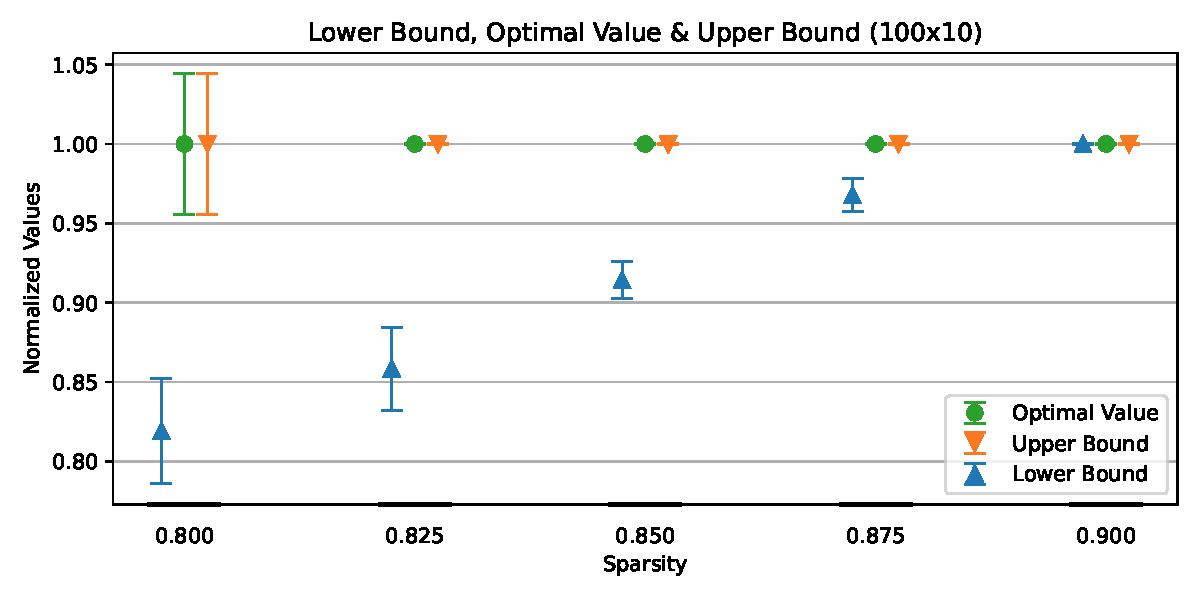
\includegraphics[scale=.787]{assets/figures/tony.pdf}
    \caption{Qualità delle limitazioni prodotte dall'algoritmo di Frank-Wolfe, normalizzate rispetto al valore ottimo
    trovato dall'algoritmo del simplesso, per matrici \( 100\times10 \).}
    \label{fig:quality_small1}
\end{figure}

\noindent Osserviamo che nonostante la dimensione ridotta della matrice, le piccole variazioni in termini di sparsità
hanno un grande effetto sulla qualità della limitazione inferiore prodotta dall'algoritmo di Frank-Wolfe. In
particolare, notiamo che l'aumentare del valore di sparsità corrisponde a un miglioramento nel valore della limitazione
inferiore, ma non ha alcun effetto sulla limitazione superiore, che coincide quasi sempre con il valore ottimo fornito
dall'algoritmo del simplesso. Inoltre, quando la sparsità è abbastanza elevata, anche la limitazione inferiore raggiunge
il valore ottimo.

Considerando matrici di riferimento \( 100\times50 \) e \( 100\times100 \), otteniamo i risultati della figura
\ref{fig:quality_small2}. In questo caso, l'aumento del numero di elementi ci ha permesso di considerare valori di
sparsità ancora più alti. Notiamo che, diversamente da quanto accadeva in precedenza, l'aumento
della sparsità non è più garanzia di un miglioramento nel valore della limitazione inferiore ma è indicatore di un
miglioramento nel valore della limitazione superiore che però, in questo caso, non è più così vicina al valore ottimo
come accadeva con matrici \( 100\times 10 \). Come prima, anche in questo caso utilizzare un valore di sparsità
sufficientemente elevato ci permette di chiudere sul valore ottimo con entrambe le limitazioni. Se invece consideriamo
valori di sparsità inferiori, le limitazioni non sono poi così buone.
\begin{figure}[h]
    \centering
    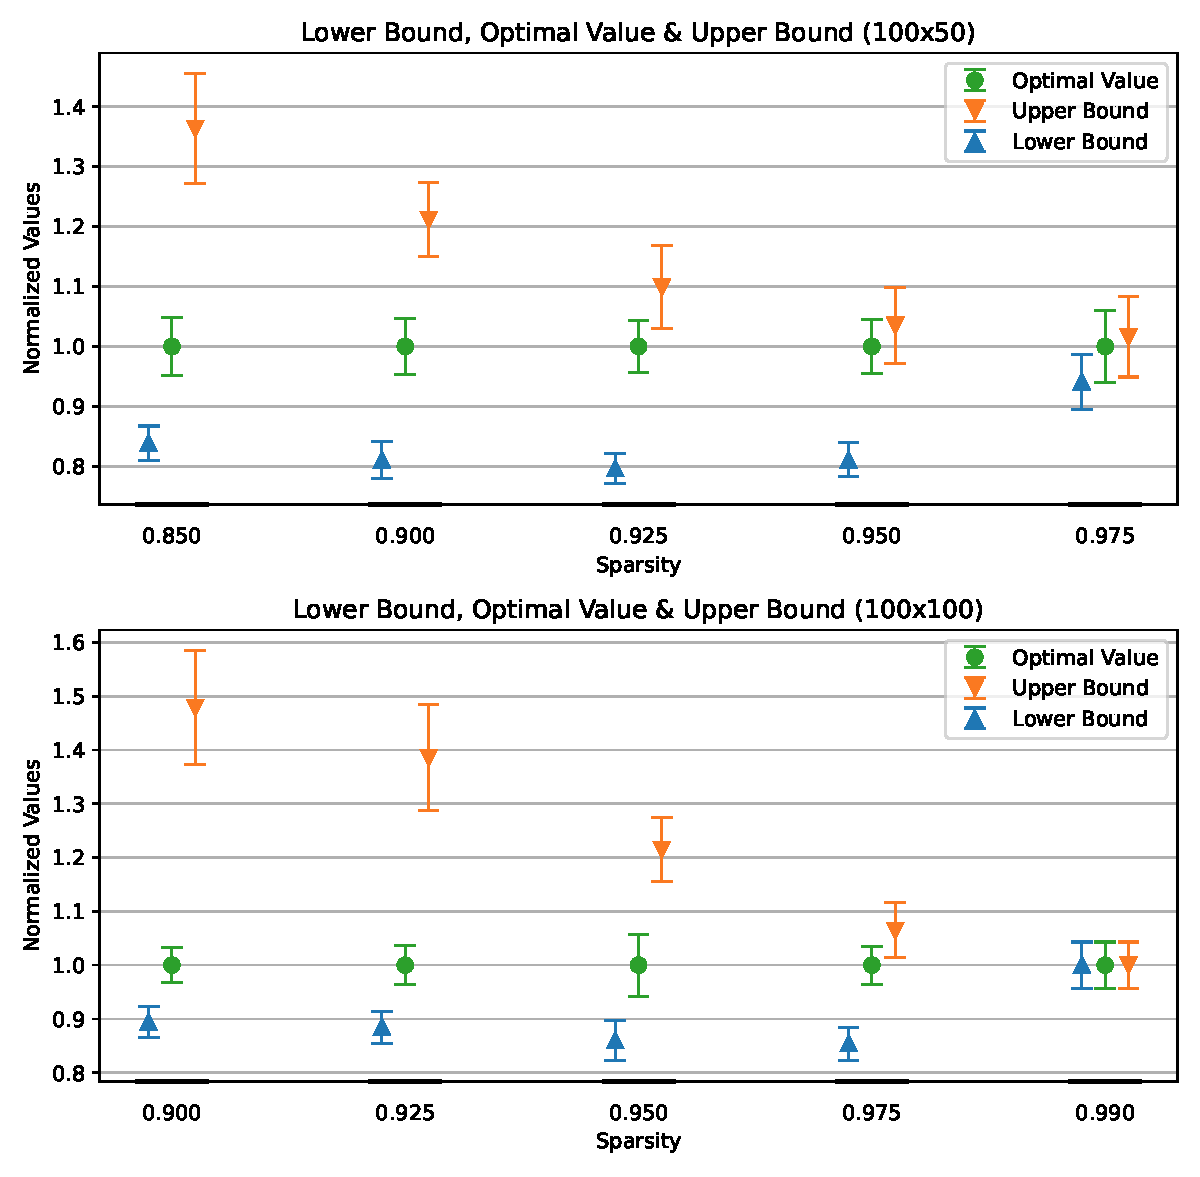
\includegraphics[scale=.787]{assets/figures/Small23.pdf}
    \caption{Qualità delle limitazioni prodotte dall'algoritmo di Frank-Wolfe, normalizzate rispetto al valore ottimo
    trovato dall'algoritmo del simplesso, per matrici \( 100\times 50 \) (sopra) e \( 100\times100 \) (sotto).}
    \label{fig:quality_small2}
\end{figure}

\noindent
In aggiunta, si osserva sperimentalmente che la qualità delle limitazioni superiori prodotte da Frank-Wolfe è
influenzata molto di più dal numero delle variabili del problema, piuttosto che dal numero degli elementi della matrice
di riferimento ad esso associata. La figura \ref{fig:quality_small_extra} mostra i risultati dell'esecuzione dei due
algoritmi su istanze aggiuntive che confermano quanto appena argomentato.
\begin{figure}[ht]
    \centering
    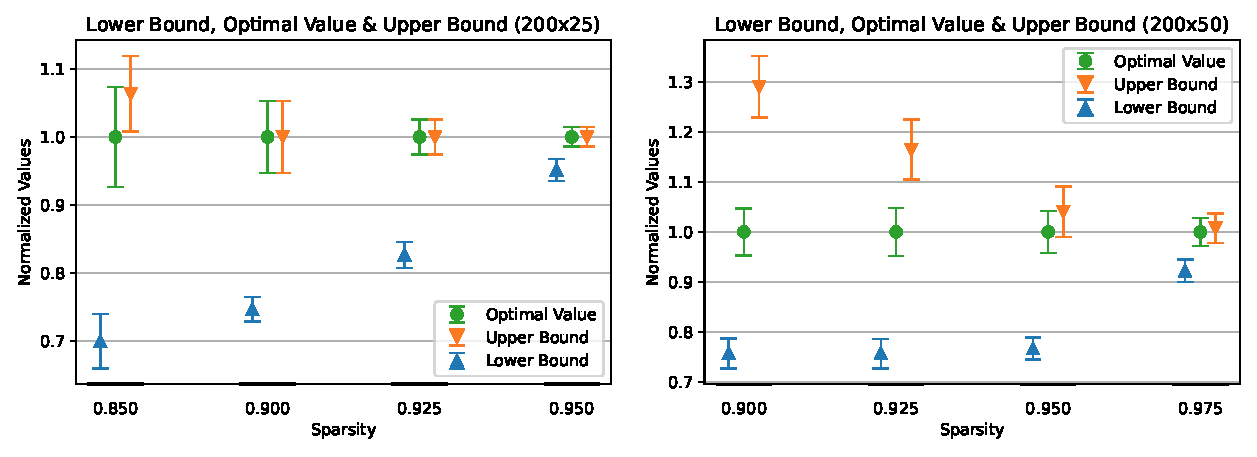
\includegraphics[width=\textwidth]{assets/figures/Extra.pdf}
    \caption{Qualità delle limitazioni prodotte dall'algoritmo di Frank-Wolfe, normalizzate rispetto al valore ottimo
    trovato dall'algoritmo del simplesso, per matrici \( 200\times 25 \) (sinistra) e \( 200\times50 \) (destra).}
    \label{fig:quality_small_extra}
\end{figure}

\noindent
Le istanze identificate da matrici \( 100\times 50 \) e \( 200\times 25 \) sono caratterizzate dallo stesso numero di
elementi, ma confrontando il grafico associato alle matrici \( 100\times 50 \) della figura \ref{fig:quality_small2} con
il grafico a sinistra della figura \ref{fig:quality_small_extra}, che si riferisce a matrici \( 200\times 25 \), si nota
immediatamente la differenza nella qualità della limitazione superiore. L'esecuzione dell'algoritmo di Frank-Wolfe sulle
istanze con un numero maggiore di variabili ha prodotto limitazioni superiori peggiori rispetto a quanto ottenuto per
istanze caratterizzate da un numero inferiore di variabili, nonostante la sparsità e il numero degli elementi delle
matrici di riferimento fosse lo stesso. Se invece ci riferiamo a istanze che hanno matrici di riferimento con lo stesso
numero di variabili, è sufficiente confrontare il grafico a destra della figura \ref{fig:quality_small_extra} con il
grafico in alto nella figura \ref{fig:quality_small2} per capire che l'aumento del numero di elementi della matrice di
riferimento non è un fattore così influente sulla qualità della limitazione superiore. Anzi, a parità di sparsità e
numero di variabili, l'aumento del numero degli elementi causa un miglioramento nella limitazione superiore. Di
conseguenza, la differenza nella qualità delle limitazioni superiori prodotte da Frank-Wolfe per le istanze con matrici
di riferimento \( 200\times 25 \) e  \( 200\times 50 \) è da attribuire alla variazione nel numero delle variabili,
piuttosto che alla variazione del numero degli elementi.

\end{document}


\section{Confronto dei tempi di esecuzione}

Iniziamo confrontando i tempi di esecuzione dei due algoritmi per istanze di taglia diversa. Abbiamo individuato tre
classi di istanze in base del numero di elementi della matrice di riferimento e per ciascuna di queste procederemo
ad eseguire i due algoritmi. Inoltre, per ciascuna classe consideriamo diversi valori di sparsità delle matrici ed effettuiamo
l'esperimento su molteplici istanze.

\subsection{Istanze di taglia piccola}
La classe di istanze di taglia piccola è costituita da istanze caratterizzate da matrici di riferimento con \( m \)
righe e
\(
    n
\)
colonne tali che il numero di elementi è \( m\times n \leq 10\,000 \).

\subsection{Istanze di taglia media}
La classe di istanze di taglia media è costituita da istanze caratterizzate da matrici di riferimento con \( m \)
righe e
\(
    n
\)
colonne tali che il numero di elementi è \( m\times n \leq 1\,000\,000 \).

\subsection{Istanze di taglia grande}
La classe di istanze di taglia grande è costituita da istanze caratterizzate da matrici di riferimento con \( m \)
righe e
\(
    n
\)
colonne tali che il numero di elementi è \( m\times n \leq 10000 \).


\newpage
\begin{figure}[h]
    \centering
    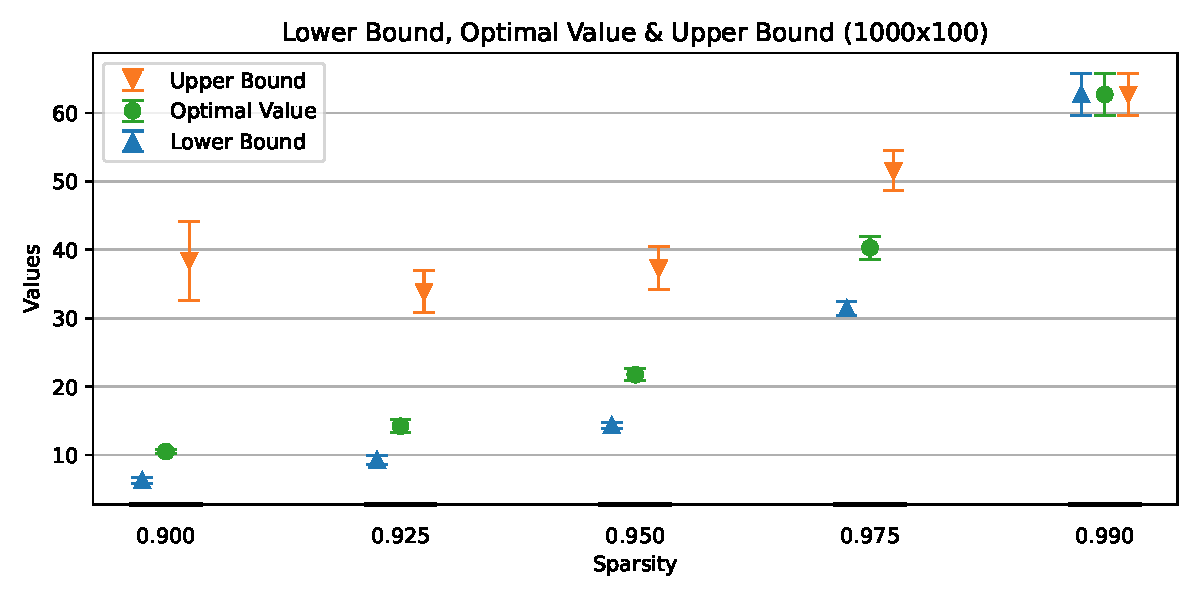
\includegraphics[scale=.787]{assets/figures/Figure_15.pdf}
    \caption{hi}
\end{figure}


L'esperimento è stato effettuato su istanze di taglia diversa per capire come variano i tempi di esecuzione al variare
del numero di elementi della matrice di riferimento. Inoltre, a parità di taglia abbiamo svolto l'esperimento su istanze
caratterizzate da matrici di riferimento con valori di sparsità differenti.



Inoltre, abbiamo analizzato la qualità della
soluzione prodotta dall'algoritmo di Frank-Wolfe al variare del numero di iterazioni, con l'obiettivo di individuare un
limite che garantisca una soluzione accettabile in un tempo ridotto.
\newpage

\section{Confronto dei tempi di esecuzione}

\subsection{Istanze di taglia piccola}

\subsection{Istanze di taglia media}

\subsection{Istanze di taglia grande}

\subsection{Sparsità della matrice di riferimento}

\section{Convergenza dell'algoritmo di Frank-Wolfe}

\subsection{Gap sul valore ottimo}

\subsection{Numero di iterazioni}


\begin{landscape}
\begin{figure}[b]
    \centering
    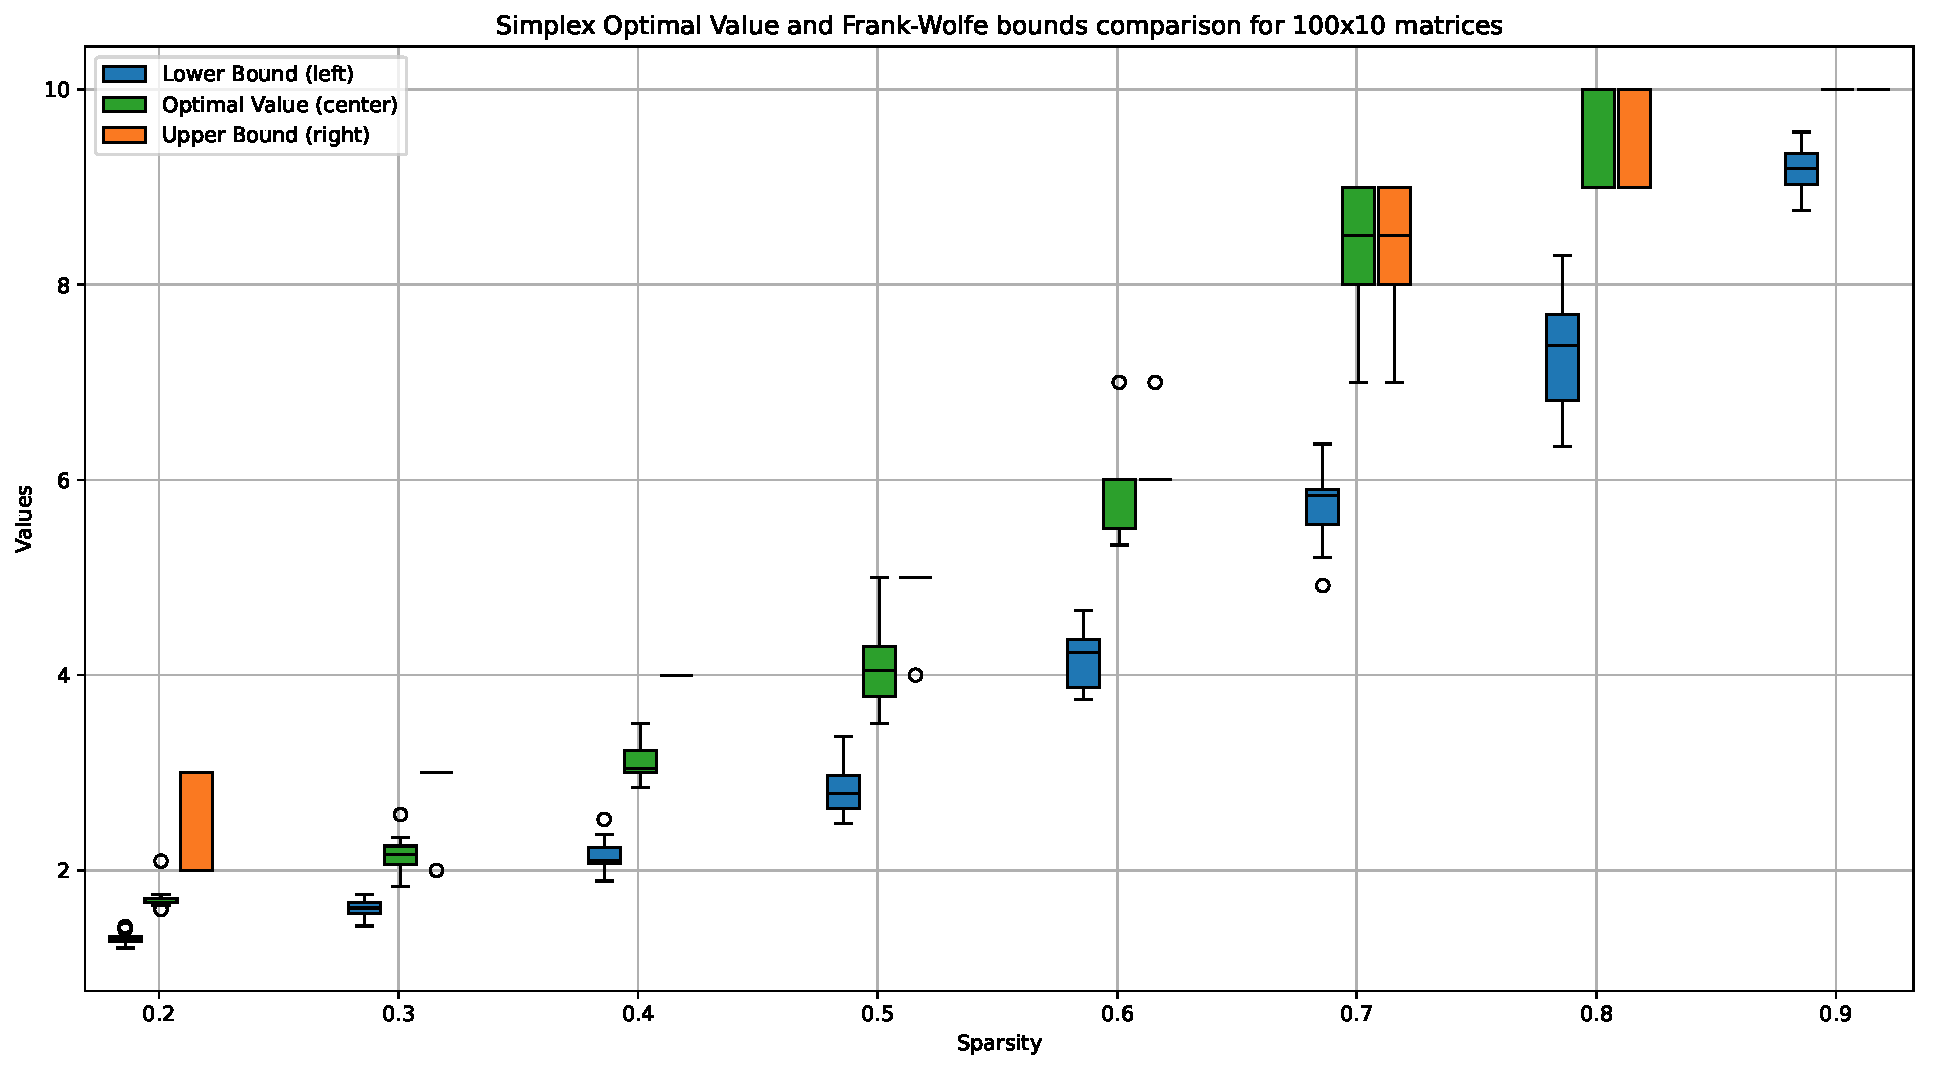
\includegraphics[scale=0.7]{assets/figures/firstactualtest.pdf}
    \caption{hi}
\end{figure}
\end{landscape}

\newpage


\begin{landscape}
\begin{table}[h]
    \centering
    \begin{tabularx}{1.35\textwidth}{XXXXccXX}
        \toprule
        && \multicolumn{2}{c}{\textbf{Simplex}} & \multicolumn{4}{c}{\textbf{Frank-Wolfe}}\\ \midrule
        \textbf{Size} & \textbf{Sparsity} & \textbf{Objective} & \textbf{Time} &
        \textbf{Lower Bound} & \textbf{Upper Bound} & \textbf{Time} & \textbf{Iterations} \\ \midrule
        10x10 & 0.2 & 8.765 & 0.456 & 7.890 & 13.585 & 0.014 \\
        \bottomrule
    \end{tabularx}
    \caption{A well-formatted table using booktabs and tabularx}
    \label{table:booktabs}
\end{table}

\end{landscape}

\newpage
\begin{landscape}
\begin{figure}[b]
    \centering
    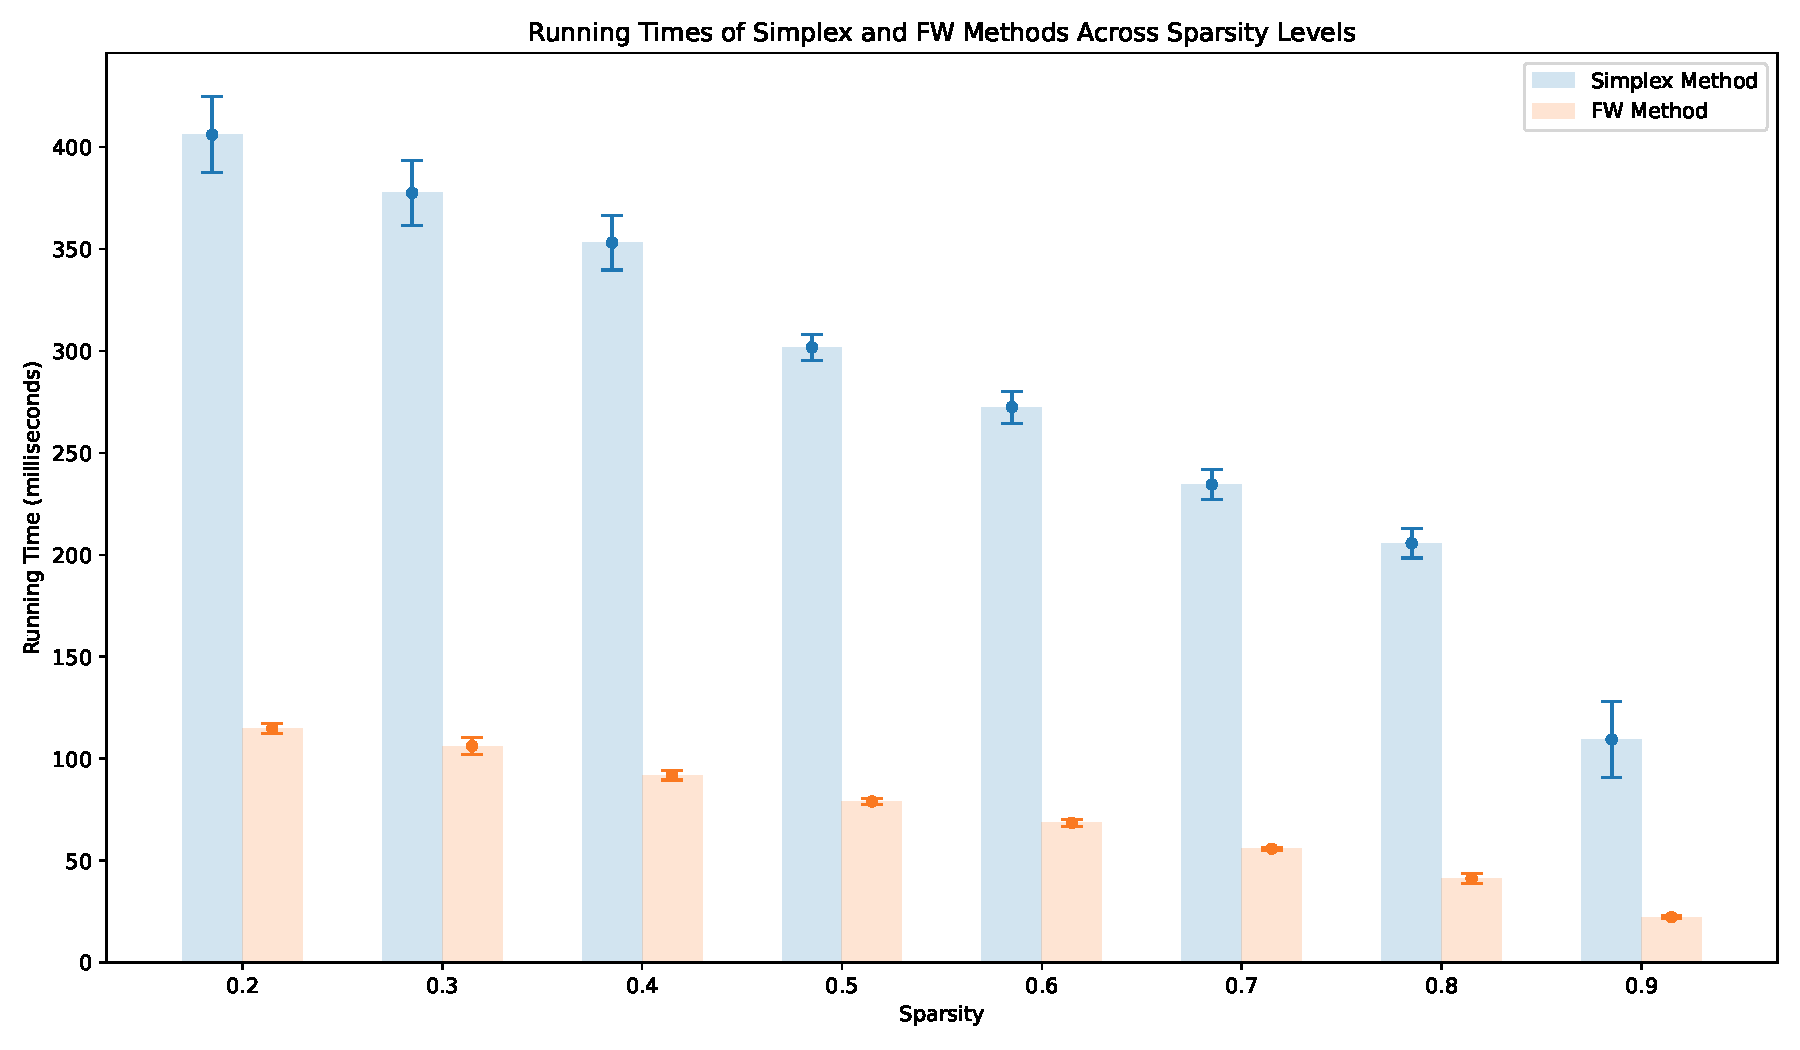
\includegraphics[scale=0.75]{assets/figures/barplot.pdf}
    \caption{hi}
\end{figure}
\end{landscape}

\newpage

%\begin{landscape}
%\begin{table}[ht]
%    \centering
%    \begin{tabularx}{\textwidth}{c c c c c c c}  % Define eight columns
%        \toprule
%        \multicolumn{2}{c}{\textbf{\alt 10$\times$10}} & \multicolumn{2}{c}{\textbf{\alt Simplesso}} &
%        \multicolumn{3}{c}{\textbf{\alt Frank-Wolfe (1000 iterazioni)}} \\
%        \cmidrule(lr){1-2} \cmidrule(lr){3-4} \cmidrule(lr){5-7}
%        \textbf{\alt Sparsità} & \textbf{\alt Istanza} & \textbf{\alt Valore Ottimo} & \textbf{\alt Tempo (ms)} &
%        \textbf{\alt Limite Inferiore} &
%        \textbf{\alt Limite Superiore} & \textbf{\alt Tempo (ms)} \\
%        \cmidrule(lr){1-2} \cmidrule(lr){3-4} \cmidrule(lr){5-7}
%        10x10 & 0.2 & 8.723382 & 0.372821 & 7.897323 & 14.328123 & 0.034123 \\
%        10x10 & 0.2 & 8.723 & 0.372 & 7.897 & 14.328 & 0.034 \\
%        10x10 & 0.2 & 8.723 & 0.372 & 7.897 & 14.328 & 0.034 \\
%        10x10 & 0.2 & 8.723 & 0.372 & 7.897 & 14.328 & 0.034 \\
%        10x10 & 0.2 & 8.723 & 0.372 & 7.897 & 14.328 & 0.034 \\
%        10x10 & 0.2 & 8.723 & 0.372 & 7.897 & 14.328 & 0.034 \\
%        10x10 & 0.2 & 8.723 & 0.372 & 7.897 & 14.328 & 0.034 \\
%        10x10 & 0.2 & 8.723 & 0.372 & 7.897 & 14.328 & 0.034 \\
%        10x10 & 0.2 & 8.723 & 0.372 & 7.897 & 14.328 & 0.034 \\
%        10x10 & 0.2 & 8.723 & 0.372 & 7.897 & 14.328 & 0.034 \\
%        \cmidrule(lr){1-2} \cmidrule(lr){3-4} \cmidrule(lr){5-7}
%        \multicolumn{2}{c}{\textbf{\alt Mediana}} & 8.723 & 0.372 & 7.897 & 14.328 & 0.034 \\
%        \multicolumn{2}{c}{\textbf{\alt Media}} & 8.723 & 0.372 & 7.897 & 14.328 & 0.034 \\
%        \multicolumn{2}{c}{\textbf{\alt Deviazione Standard}} & 8.723 & 0.372 & 7.897 & 14.328 & 0.034 \\
%        \bottomrule
%    \end{tabularx}
%    \caption{Comparison of Simplex and Frank-Wolfe methods}
%    \label{table:comparison}
%\end{table}
%\end{landscape}

\newpage
\begin{table}[ht]
    \centering
    \begin{tabularx}{386.53947pt}{ccccc}  % Define eight columns
        \toprule
        & \multicolumn{2}{c}{\text{\alt Simplesso (ms)}} & \multicolumn{2}{c}{\text{\alt Frank-Wolfe (ms)}} \\
        \cmidrule(lr){2-3} \cmidrule(lr){4-5}
        \text{\alt Sparsità} &  \text{\alt Media} & \text{\alt Deviazione Standard}
        & \text{\alt Media} & \text{\alt Deviazione Standard} \\
        \cmidrule(lr){1-1} \cmidrule(lr){2-3} \cmidrule(lr){4-5}
        0.2 & 406.146 & 18.793 & 114.911 & 2.456 \\
        0.3 & 377.539 & 16.088 & 106.234 & 4.256 \\
        0.4 & 353.128 & 13.376 & 91.993 & 2.444 \\
        0.5 & 301.810 & 6.420 & 78.984 & 1.530 \\
        0.6 & 272.485 & 7.833 & 68.542 & 1.861 \\
        0.7 & 234.555 & 7.172 & 55.862 & 0.770 \\
        0.8 & 205.662 & 7.182 & 41.336 & 2.501 \\
        0.9 & 109.421 & 18.446 & 22.232 & 0.700 \\
        \bottomrule
    \end{tabularx}
    \caption{Confronto dei tempi (medi) di esecuzione dell'algoritmo del simplesso e dell'algoritmo di Frank-Wolfe per
    istanze 1000x100. L'algoritmo di Frank-Wolfe termina dopo 1000 iterazioni.}
    \label{table:comparidsson}
\end{table}
